%% Chapter 4: Results and Analysis (Part I): chapters/chapter04.tex

% ==============================================================================
% Chapter Guidelines & Content Description:
% - Presentation of primary research results (structural, electronic).
% - Structured tables using booktabs package.
% - Interactive data plots using pgfplots package.
% ==============================================================================

\chapter{Results and Analysis (Part I): Structural and Electronic Properties}
\label{ch:results_1}

\section{Structural Relaxation}
First-principles structural relaxation was performed for bulk and monolayer configurations. The optimized lattice parameters, compared with experimental values, are summarized in Table~\ref{tab:structural_relax}.

\begin{table}[H]
    \centering
    \caption{Optimized lattice parameters ($a$ and $c$ in \si{\angstrom}) and bulk modulus ($B_0$ in \si{\giga\pascal}) compared with experimental literature.}
    \label{tab:structural_relax}
    \begin{tabular}{l c c c c c}
        \toprule
        \multirow{2}{*}{\textbf{Material}} & \multicolumn{2}{c}{\textbf{Calculated (DFT-GGA)}} & \multicolumn{2}{c}{\textbf{Experimental}} & \multirow{2}{*}{$B_0$ (GPa)} \\
        \cmidrule(r){2-3} \cmidrule(l){4-5}
        & $a$ & $c$ & $a$ & $c$ & \\
        \midrule
        MoS$_2$ (Bulk)  & 3.185 & 12.352 & 3.160 & 12.290 & 53.2 \\
        MoSe$_2$ (Bulk) & 3.321 & 12.980 & 3.299 & 12.901 & 47.8 \\
        WS$_2$ (Bulk)   & 3.182 & 12.420 & 3.153 & 12.300 & 62.1 \\
        WSe$_2$ (Bulk)  & 3.318 & 13.012 & 3.282 & 12.960 & 55.4 \\
        \bottomrule
    \end{tabular}
\end{table}

\section{Electronic Bandgap Tuning under Strain}
The dependence of the electronic bandgap on biaxial tensile and compressive strain was investigated. The results are plotted in Figure~\ref{fig:bandgap_strain}.

\begin{figure}[H]
    \centering
    \begin{subfigure}[b]{0.75\textwidth}
        \centering
        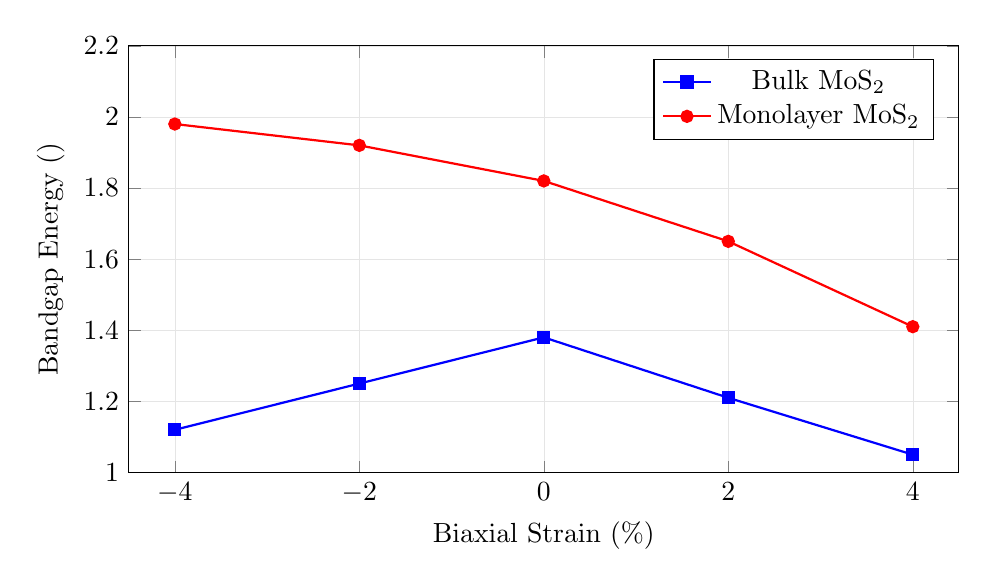
\begin{tikzpicture}
            \begin{axis}[
                width=\textwidth,
                height=7cm,
                xlabel={Biaxial Strain (\%)},
                ylabel={Bandgap Energy (\si{\electronvolt})},
                xmin=-4.5, xmax=4.5,
                ymin=1.0, ymax=2.2,
                xtick={-4,-2,0,2,4},
                ytick={1.0,1.2,1.4,1.6,1.8,2.0,2.2},
                legend pos=north east,
                grid=both,
                grid style={line width=.1pt, draw=gray!10},
                major grid style={line width=.2pt, draw=gray!20}
            ]
                % Bulk MoS2
                \addplot[
                    color=blue,
                    mark=square*,
                    thick
                ]
                coordinates {
                    (-4,1.12) (-2,1.25) (0,1.38) (2,1.21) (4,1.05)
                };
                \addlegendentry{Bulk MoS$_2$}
                
                % Monolayer MoS2
                \addplot[
                    color=red,
                    mark=otimes*,
                    thick
                ]
                coordinates {
                    (-4,1.98) (-2,1.92) (0,1.82) (2,1.65) (4,1.41)
                };
                \addlegendentry{Monolayer MoS$_2$}
            \end{axis}
        \end{tikzpicture}
    \end{subfigure}
    \caption{Tuning of electronic bandgap of bulk and monolayer MoS$_2$ as a function of biaxial strain.}
    \label{fig:bandgap_strain}
\end{figure}

Compressive strain is found to increase the bandgap in monolayer systems up to 2\% strain, beyond which it decreases due to a change in the valence band maximum (VBM) state symmetry.
